\chapter{PROJECT BUDGET}
\label{app:project_budget}

The proposed system is mainly a software and research project. Most tools and datasets are free or open source, so the budget is focused on internet access, optional computing resources, hosting, printing, binding, and miscellaneous project expenses.

\begin{table}[H]
    \centering
    \small
    \caption{Estimated Project Budget}
    \label{tab:appendix_project_budget}
    \begin{tabularx}{0.94\linewidth}{|p{3.2cm}|X|p{2.8cm}|}
        \hline
        \textbf{Category} & \textbf{Description} & \textbf{Estimated Cost} \\
        \hline
        Internet and data access & Dataset downloads, API access, research review, and collaboration & NRs. 2,000 \\
        \hline
        Cloud/GPU usage & Optional Google Colab Pro, Kaggle, or equivalent compute for model training & NRs. 5,000 \\
        \hline
        Domain or hosting & Optional dashboard deployment for demonstration & NRs. 3,000 \\
        \hline
        Printing and binding & Mid-term report, final report, and presentation materials & NRs. 6,000 \\
        \hline
        Miscellaneous & Backup storage and unforeseen project needs & NRs. 2,000 \\
        \hline
        \multicolumn{2}{|r|}{\textbf{Total Estimated Cost}} & \textbf{NRs. 18,000} \\
        \hline
    \end{tabularx}
\end{table}

\chapter{PROJECT TIMELINE}
\label{app:project_timeline}

The project is planned in phases: literature review, dataset preparation, preprocessing, graph construction, baseline modeling, GAT-GRU implementation, explainability, dashboard development, testing, and final documentation.

\begin{figure}[H]
    \centering
    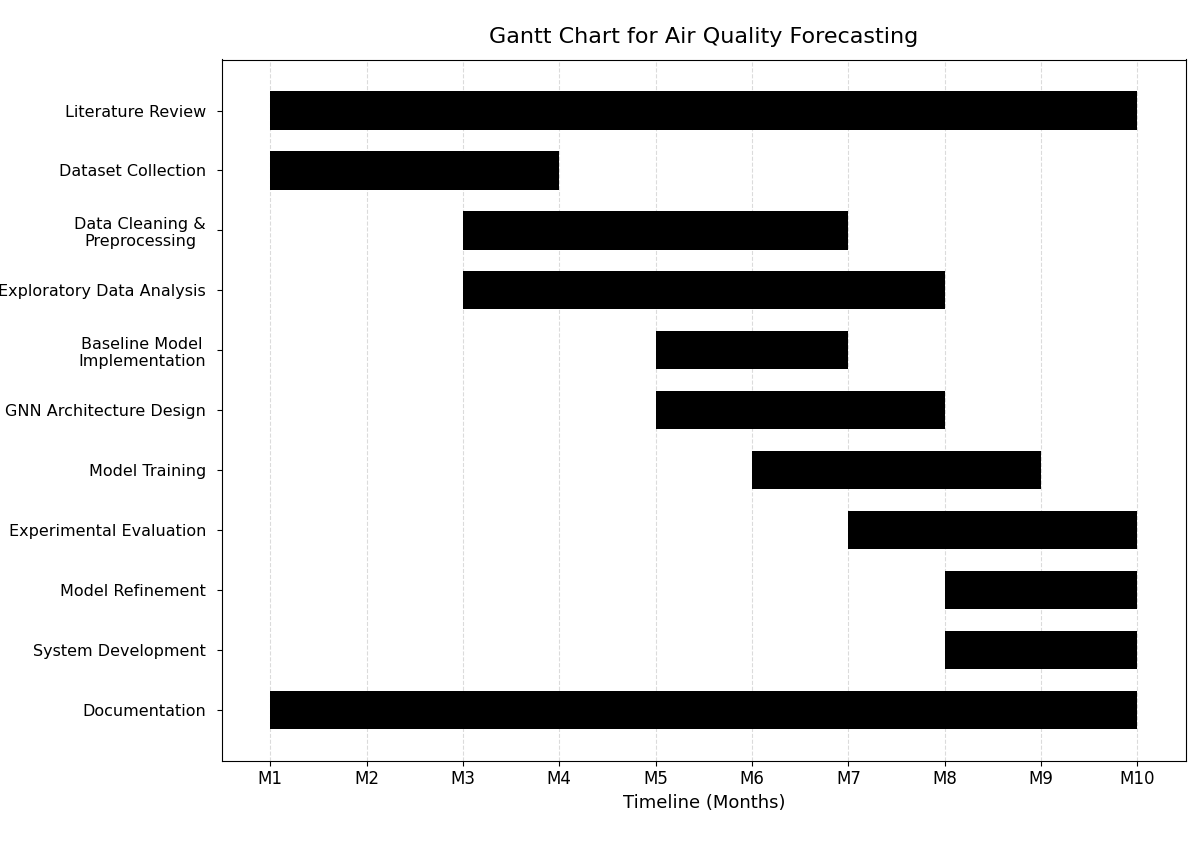
\includegraphics[width=\textwidth]{src/images/figures/gantt_chart.png}
    \caption{Project Gantt Chart}
    \label{fig:appendix_gantt_chart}
\end{figure}

\chapter{DATASET DETAILS}
\label{app:dataset_details}

The dataset for this project contains station-wise PM$_{2.5}$ observations and meteorological variables aligned at an hourly resolution. The major fields include timestamp, station name, station coordinates, PM$_{2.5}$, PM$_1$, temperature, humidity, pressure, dew point, wind speed, wind direction, and temporal features. The final cleaned dataset will be used to generate sliding-window inputs for short-term PM$_{2.5}$ forecasting.

\begin{table}[H]
    \centering
    \small
    \caption{Dataset Field Description}
    \label{tab:dataset_field_description}
    \begin{tabularx}{0.94\linewidth}{|p{3.6cm}|X|}
        \hline
        \textbf{Field} & \textbf{Description} \\
        \hline
        Timestamp & Hourly time index used to synchronize air quality and weather records \\
        \hline
        Station metadata & Station name, station identifier, latitude, and longitude \\
        \hline
        Pollutant features & PM$_{2.5}$ target variable and available pollutant inputs such as PM$_1$ \\
        \hline
        Meteorological features & Temperature, relative humidity, pressure, dew point, wind speed, and wind direction \\
        \hline
        Temporal features & Hour of day, day of week, month, and season for periodic behavior modeling \\
        \hline
        Missingness indicators & Optional binary indicators showing whether values were observed or imputed \\
        \hline
    \end{tabularx}
\end{table}
